\chapter{Confronto dati}
\section{Angolo di stallo}
Il numero di Reynolds della prova è particolarmente basso, per questo motivo polari sperimentali affidabili non sono presenti in letteratura. Per ovviare a ciò è stata calcolata numericamente la porzione del grafico $Cl-\alpha$ per angoli compresi tra 8° e 12° (con passo 1°), il calcolo è stato effettuato con \emph{Ansys Fluent} utilizzando $k-\omega SST$ come modello di turbolenza. Il massimo $C_p$ è stato ottenuto ad 11°, l'angolo di stallo numerico sarà quindi compreso tra i 10° e i 12°, il risultato è concorde con quanto osservato nella visualizzazione [fig: \ref{erostall} ].
\section{Numero di Strouhal}
Non sono state reperite prove sperimentali comparabili all'esperimento qui considerato, ma la condizione fortemente stallata esibita durante le acquisizione consente di paragonare il profilo ad un corpo tozzo. \\
A riguardo la letteratura è ricca di prove sperimentali eseguite sul corpo tozzo per eccellenza: il cilindro. \\

\begin{figure}[h]
\centering
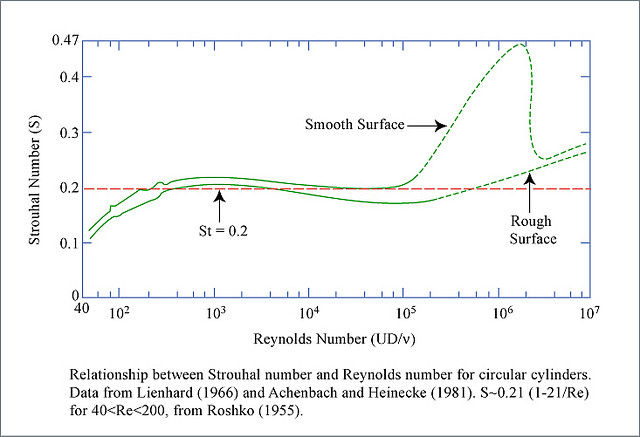
\includegraphics[scale=0.35]{Figure/str.jpg}
\caption{Numero di Strouhal nel cilindro}
\label{fig: Numero di Strouhal nel cilindro}
\end{figure}
Si può quindi assumere un numero di Strouhal pari a 0.2 [fig: \ref{fig: Numero di Strouhal nel cilindro}].

\begin{table}[h]
\centering
\begin{tabular}{|c|c|c|c|}
\hline
Strouhal teorico & Acquisizione 1 & Acquisizione 2 & Acquisizione 3\\
\hline
%$0.2$  & $0.222 \pm 0.004$   & $0.205 \pm 0.011$ & $0.194 \pm 0.011$\\
$0.2$  & $0.222$   & $0.205 $ & $0.194 $\\
\hline
\end{tabular}
\caption{Confronto numero Strouhal}
\label{tab: Confronto numero Strouhal}
\end{table}

Si nota come la seconda e la terza acquisizione [tab: \ref{tab: Confronto numero Strouhal} ] diano riscontro con il valore atteso; la prima,probabilmente a casua dell'incidenza minore, sovrastima il numero di Strouhal di oltre il dieci percento.

\section{Campo di moto e spessore scia}
E' stata eseguita una simulazione numerica nelle condizioni della prova [fig: \ref{fig: Campo di moto Fluent} ]. Il sotware utilizzato è \emph{Ansys Fluent},la mesh è dimensionata per riprodurre le dimensioni della camera di prova e, visto l'angolo di incidenza ridotta, è stato usato il modello di turbolenza ad 1 equazione di \emph{Spalart-Allmaras}. 

\begin{figure}[H]
\centering
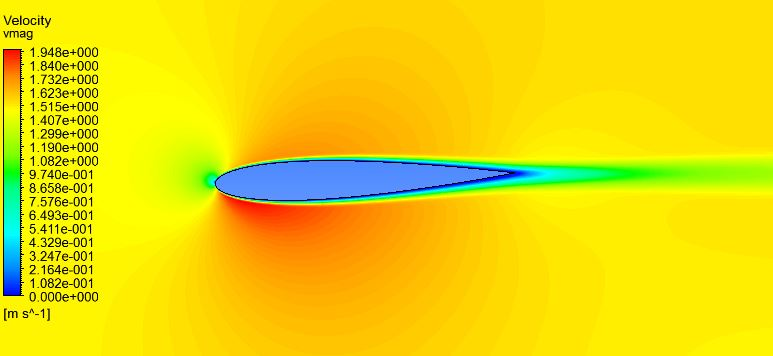
\includegraphics[scale=0.7]{Figure/CFD_wake.JPG}
\caption{Campo di moto calcolato con Fluent}
\label{fig: Campo di moto Fluent}
%\end{figure}

%\begin{figure}[h!]
\centering
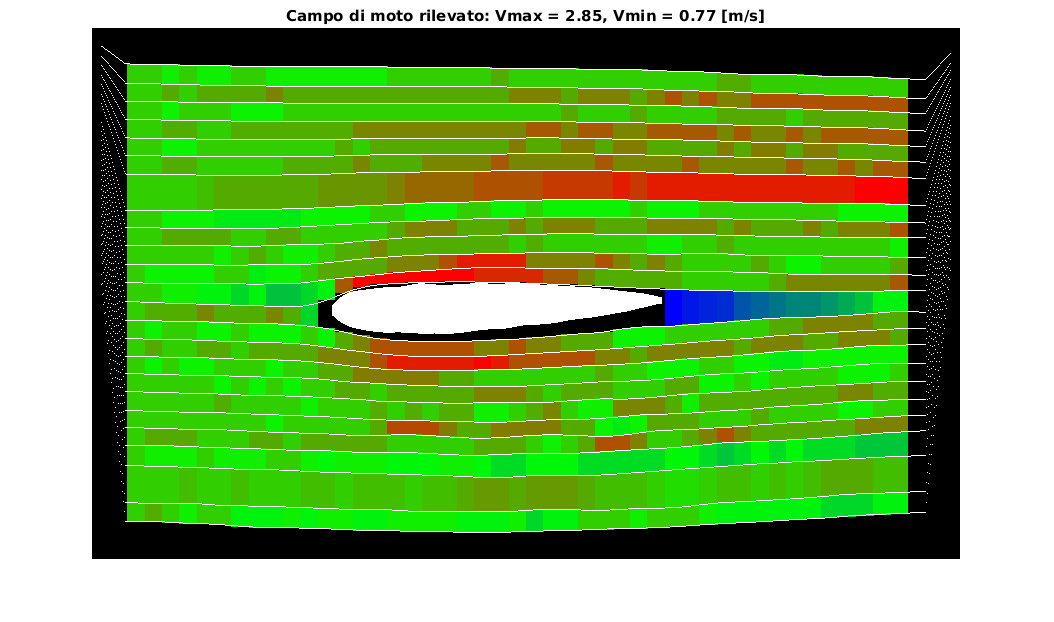
\includegraphics[scale=0.6]{Figure/v_field.png}
\caption{Campo di velocità calcolato da acquisizioni}
\label{fig: Campo di velocità calcolato}
\end{figure}

Il campo di moto simulato è stato campionato nelle coordinate ottenute dalla visualizzazione [fig \ref{fig: Campo di velocità calcolato} ], l'errore medio rilevato è 0.3 \emph{m/s}, con picchi di oltre $ 1 \emph{m/s}$. Da un confronto delle linee di corrente si nota che l'immagine elaborata è ancora distorta e,probabilmente, con un allineamento non perfetto nella fotocamera [fig: \ref{fig: Confronto linee di corrente}]. La distorsione è maggiore nella parte destra dell'immagine dove infatti si calcolano velocità non coerenti con il campo di moto: in particolare l'estremo destro del settimo tubo di flusso fa registrare una delle velocità più elevate dell'intero campo calcolato. 


\begin{figure}[H]
\centering
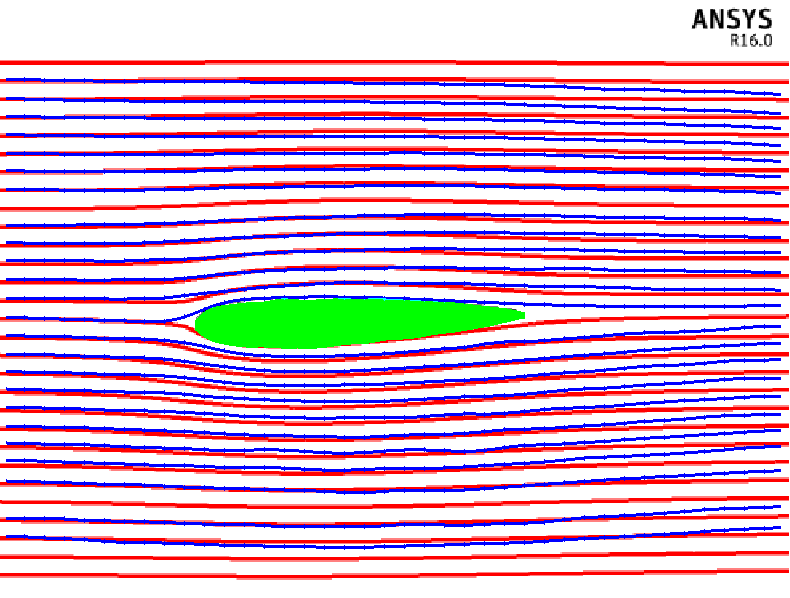
\includegraphics[scale=0.73]{Figure/Confronto.png}
\caption{Confronto linee di corrente Fluent (rosso) e linee di corrente acquisite (blu)}
\label{fig: Confronto linee di corrente}
\end{figure}


\begin{figure}[H]
\centering
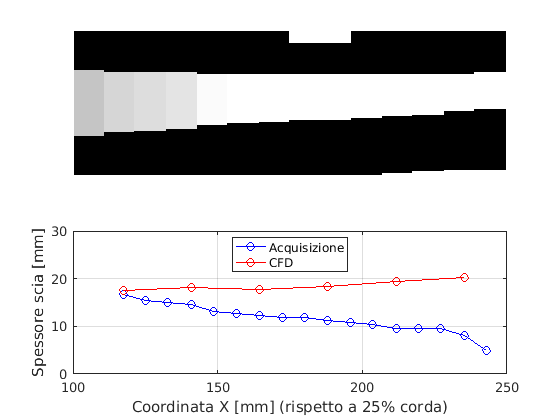
\includegraphics[scale=0.9]{Figure/scia_sper.png}
%\caption{Post interpolazione e filtraggio}
\caption{Scia visualizzata e andamento lungo coordinata X }
\label{fig: Scia rilevata}
\end{figure}

Stesso procedimento è stato effettuato per la scia, si nota che lo spessore oltre avere media quasi doppia ha anche un andamento opposto [fig: \ref{fig: Scia rilevata} ].\\

%t_{wake,video} = 11.61 \pm 3.9 [mm]
\begin{center}
$$ < t_{wake,video}(x) > = 11  [mm] $$
$$ < t_{wake,CFD}(x) >   = 18  [mm] $$
\end{center}

